%%%%%%%%%%%%%%%%%%%%%%%%%%%%%%%%%%%%%%%%%
% Beamer Presentation
% LaTeX Template
% Version 1.0 (10/11/12)
%
% This template has been downloaded from:
% http://www.LaTeXTemplates.com
%
% License:
% CC BY-NC-SA 3.0 (http://creativecommons.org/licenses/by-nc-sa/3.0/)
%
%%%%%%%%%%%%%%%%%%%%%%%%%%%%%%%%%%%%%%%%%

%----------------------------------------------------------------------------------------
%	PACKAGES AND THEMES
%----------------------------------------------------------------------------------------

\documentclass{beamer}

\mode<presentation> {

% The Beamer class comes with a number of default slide themes
% which change the colors and layouts of slides. Below this is a list
% of all the themes, uncomment each in turn to see what they look like.

%\usetheme{default}
%\usetheme{AnnArbor}
%\usetheme{Antibes}
%\usetheme{Bergen}
%\usetheme{Berkeley}
%\usetheme{Berlin}
%\usetheme{Boadilla}
%\usetheme{CambridgeUS}
%\usetheme{Copenhagen}
%\usetheme{Darmstadt}
%\usetheme{Dresden}
%\usetheme{Frankfurt}
%\usetheme{Goettingen}
%\usetheme{Hannover}
%\usetheme{Ilmenau}
%\usetheme{JuanLesPins}
%\usetheme{Luebeck}
%\usetheme{Madrid}
%\usetheme{Malmoe}
%\usetheme{Marburg}
%\usetheme{Montpellier}
%\usetheme{PaloAlto}
%\usetheme{Pittsburgh}
%\usetheme{Rochester}
%\usetheme{Singapore}
%\usetheme{Szeged}
%\usetheme{Warsaw}
\usetheme[secheader]{Boadilla}

% As well as themes, the Beamer class has a number of color themes
% for any slide theme. Uncomment each of these in turn to see how it
% changes the colors of your current slide theme.

%\usecolortheme{albatross}
%\usecolortheme{beaver}
%\usecolortheme{beetle}
%\usecolortheme{crane}
%\usecolortheme{dolphin}
%\usecolortheme{dove}
%\usecolortheme{fly}
%\usecolortheme{lily}
%\usecolortheme{orchid}
%\usecolortheme{rose}
%\usecolortheme{seagull}
%\usecolortheme{seahorse}
%\usecolortheme{whale}
%\usecolortheme{wolverine}

%\setbeamertemplate{footline} % To remove the footer line in all slides uncomment this line
%\setbeamertemplate{footline}[page number] % To replace the footer line in all slides with a simple slide count uncomment this line

\setbeamertemplate{navigation symbols}{} % To remove the navigation symbols from the bottom of all slides uncomment this line
}

\usepackage{graphicx} % Allows including images
\usepackage{tikz}
\usepackage{booktabs} % Allows the use of \toprule, \midrule and \bottomrule in tables
\usepackage[font=small,skip=0pt]{caption}
\usepackage{cancel}


\newcommand\parallelcontent[2]{
	\begin{columns}[t]
		\column{0.65\textwidth} #1
		\column{0.35\textwidth} #2
	\end{columns}
}
\newcommand\parallelitem[2]{
	\parallelcontent
	{\begin{itemize} \item #1 \end{itemize}}
	{\begin{itemize} \item #2 \end{itemize}}
}


%----------------------------------------------------------------------------------------
%	TITLE PAGE
%----------------------------------------------------------------------------------------
%\logo{
\includegraphics[width=0.05\textwidth]{../images/utlogo}}
\title[EMC A=3]{EMC Effect for A=3 } % The short title appears at the bottom of every slide, the full title is only on the title page

\author{Jason Bane} % Your name
\institute[UTK] % Your institution as it will appear on the bottom of every slide, may be shorthand to save space
{
University of Tennessee \\ % Your institution for the title page
\medskip
\textit{jbane1@vols.utk.edu} % Your email address
}
\date{\today} % Date, can be changed to a custom date
\captionsetup{font=small,skip=0pt}
\begin{document}


\begin{frame}
	\titlepage % Print the title page as the first slide
\end{frame}

\addtobeamertemplate{frametitle}{}{%
\begin{tikzpicture}[remember picture,overlay]
\node[anchor=north east,yshift=2pt] at (current page.north east) {
\includegraphics[height=0.8cm]{../images/utlogo}};
\end{tikzpicture}}


\begin{frame}{Outline}
 % Table of contents slide, comment this block out to remove it
	\tableofcontents % Throughout your presentation, if you choose to use \section{} and \subsection{} commands, these will automatically be printed on this slide as an overview of your presentation
\end{frame}

%----------------------------------------------------------------------------------------
%	PRESENTATION SLIDES
%----------------------------------------------------------------------------------------

%------------------------------------------------
\section{EMC Effect} % Sections can be created in order to organize your presentation into discrete blocks, all sections and subsections are automatically printed in the table of contents as an overview of the talk
%------------------------------------------------

%\subsection{} % A subsection can be created just before a set of slides with a common theme to further break down your presentation into chunks

\begin{frame}{EMC Effect}
	\begin{columns}[c] % The "c" option specifies centered vertical alignment while the "t" option is used for top vertical alignment

		\column{.55\textwidth} % Left column and width
		\vspace{-15pt}
		\begin{block}{}
			European Muon Collaboration's (EMC) 1983  results for the lepton scattering experiment on Iron and Deuterium. 
			\begin{itemize}
				\item Nucleon Structure Functions
				\item Sea-Quark Distributions 
				\item Gluon Distributions 
				\item Expected $ F_A = NF_2^N + ZF_2^P $
				\item Because the binding energies of the nucleons are several orders of magnitude smaller then the momentum transfer for an interaction in DIS region
				\item Fermi interaction causing differentiation at high momentum transfer.
			\end{itemize}
		\end{block}

		\column{.45\textwidth} % Right column and width
	
		\begin{figure}
			\caption{\label{EMC} EMC data of $ F_2^{Fe}/F_2^{D}$  from 1982 \cite{cc}.}
	 		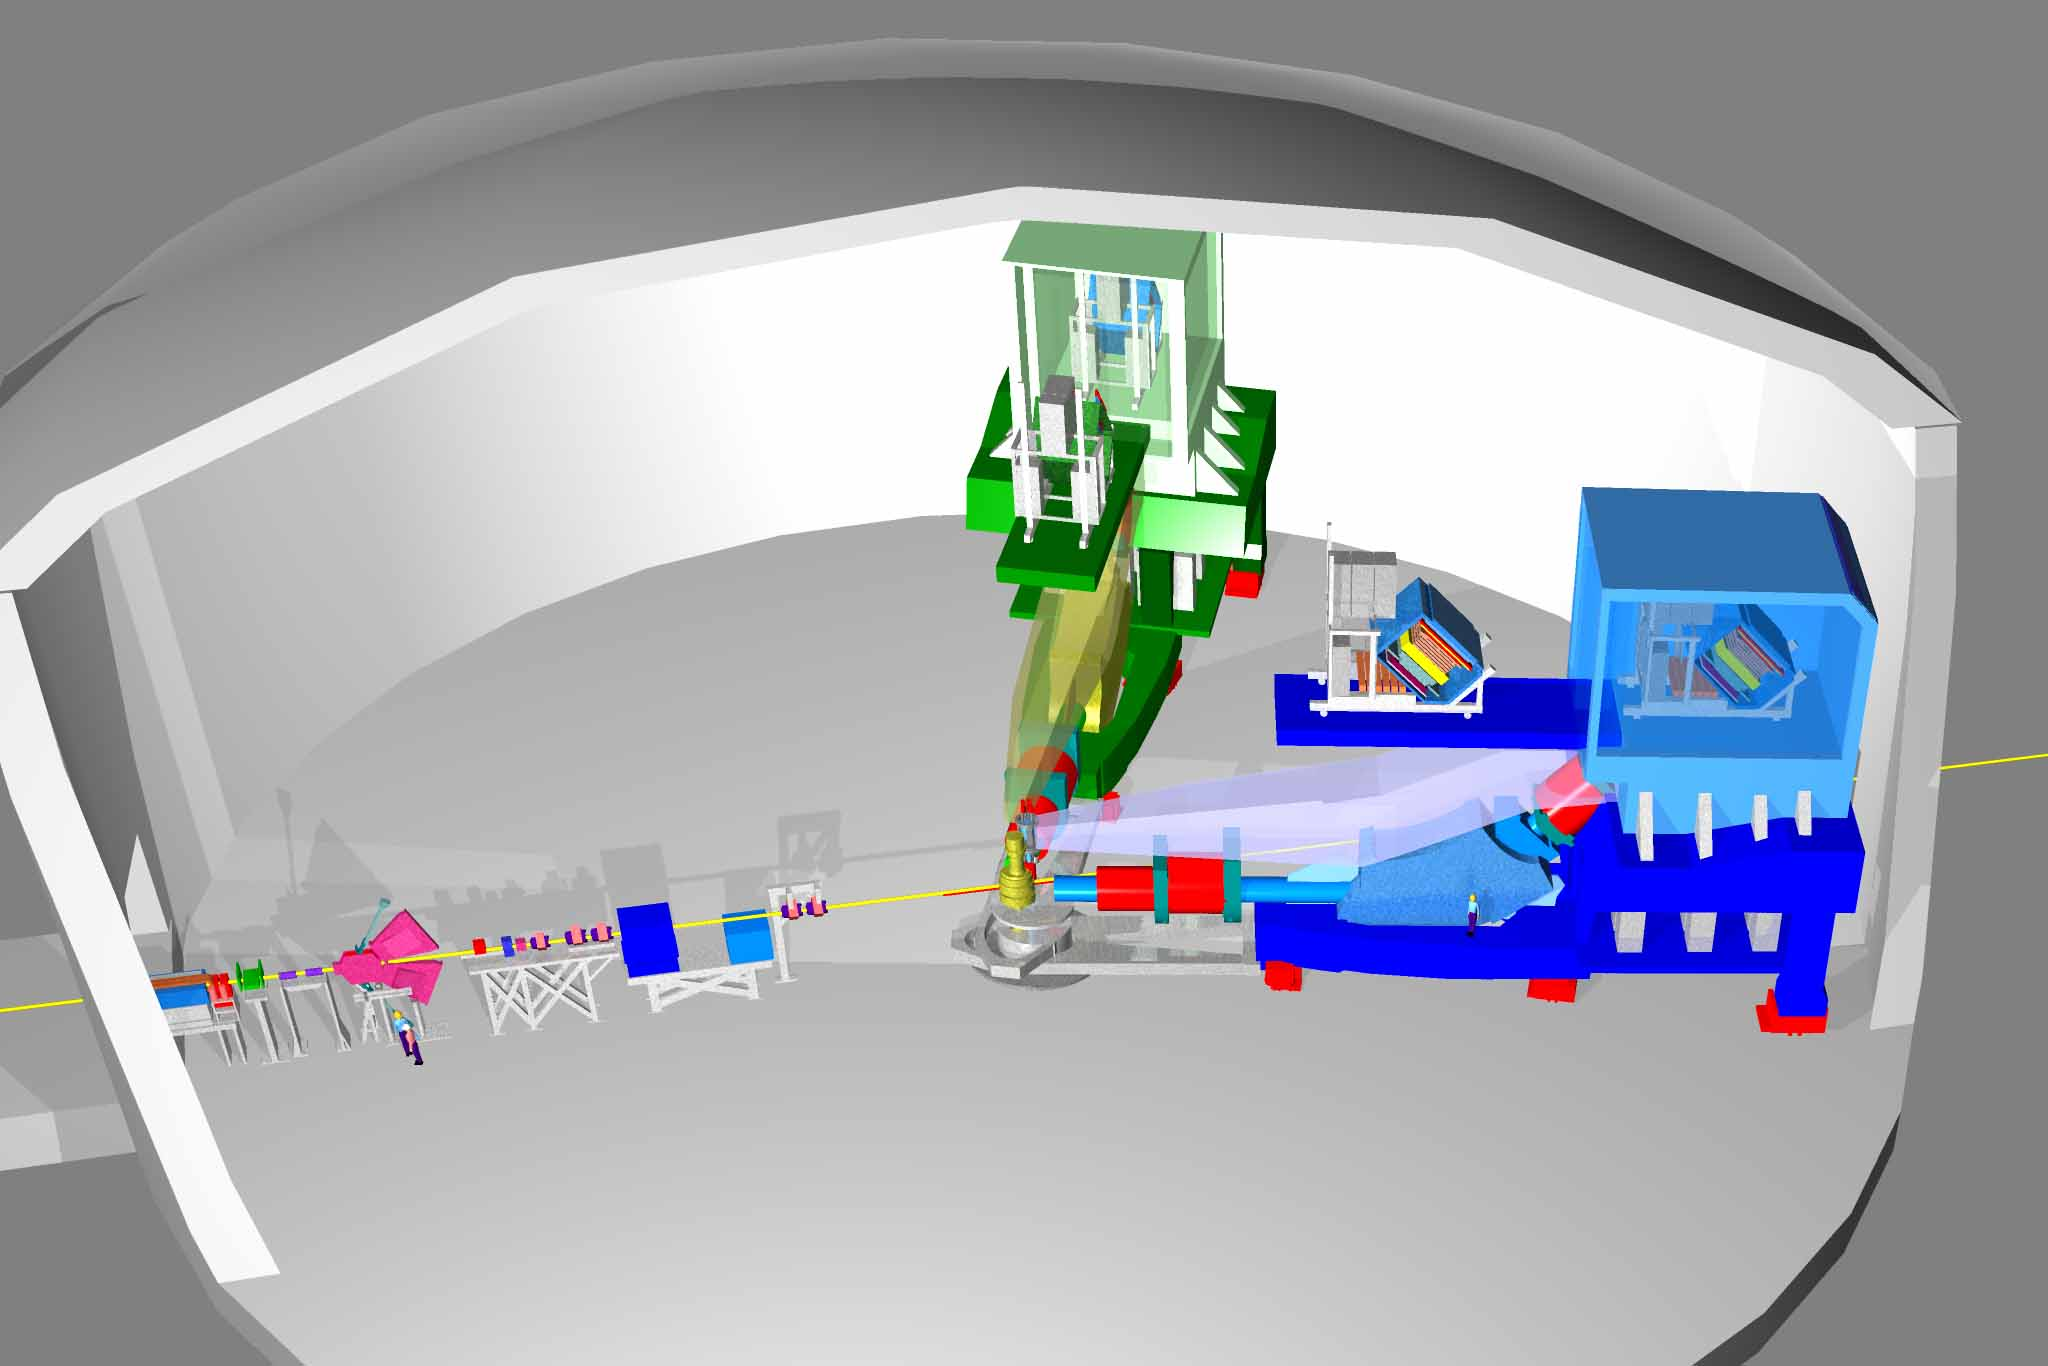
\includegraphics[width =5.5cm]{../images/EMC_cc.jpg}
	 	\end{figure}
 	\end{columns}
\end{frame}

%------------------------------------------------
\begin{frame}{EMC Effect}
	\vspace{-10pt}
	\begin{block}{}
		European Muon Collaboration:
		\begin{itemize}
			\item  Nuclear F2 structure function per nucleon different than that of deuterium
			\item Quark distribution functions modified in the nuclear medium
			\item Defined the magnitude of the EMC effect as the slope of the $\frac{A}{D}$ per nucleon cross section ratio from 0.3 to 0.7 in x.
			\item Current Explanations
			\begin{itemize}
				\item Binding effects beyond nucleon Fermi motion
				\item Enhancement of pion field with increasing A
				\item Influence of possible multi-quark clusters
				\item Change in the quark confinement scale in nuclei
			\end{itemize}
			\item No unique/universally accepted theory for explanation of effect up to date. 
		\end{itemize}
	\end{block}
\end{frame}

%----------------------------------------------
\begin{frame}{EMC Effect}

	\begin{figure}
		\caption{\label{EMC_slac} SLAC experiment E139 \cite{slac_emc}.}
		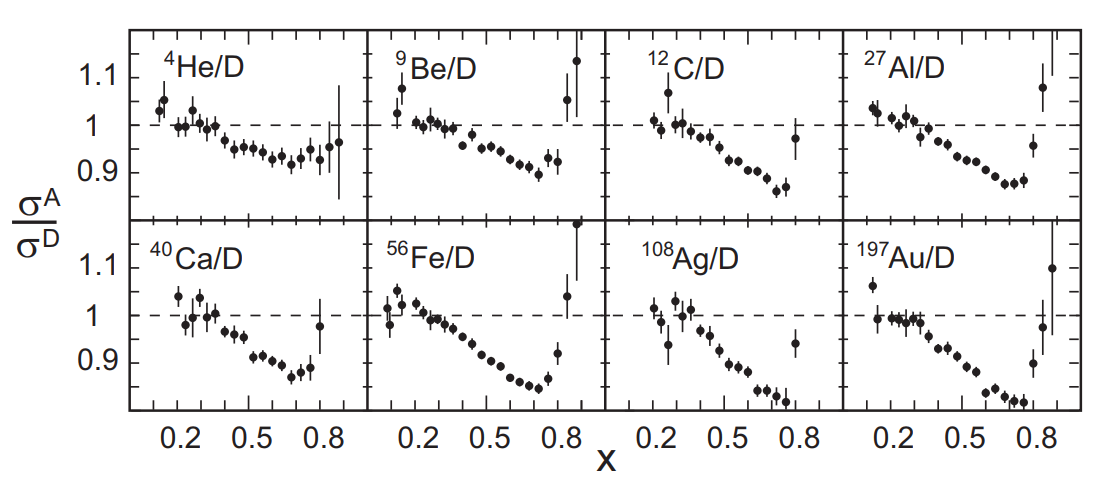
\includegraphics[width =12cm]{../images/EMC_slac_horiz.png}
	\end{figure}
	

\end{frame}

%----------------------------------------------
\begin{frame}{EMC Effect}
	\begin{columns}
		\column{.5\textwidth} % Left column and width
		\vspace{-15pt}
		\begin{figure}
			\caption{\label{E03103} JLab experiment "EMC in light Nuclei" \cite{E3103}.}
			\vspace{-20pt}
			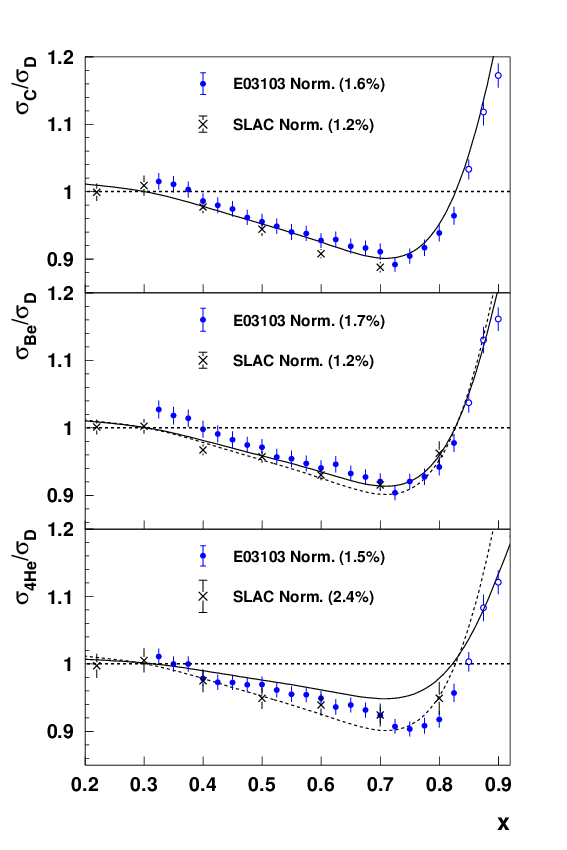
\includegraphics[width =5cm]{../images/carbon_be_he4}
		\end{figure}
		\column{.55\textwidth} % Left column and width
		\hspace{10pt}
		\begin{figure}
			\caption{\label{E03103_1} EMC as a function of Nuclear Density \cite{E3103}.}
			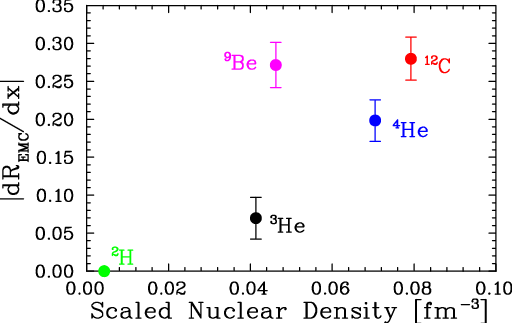
\includegraphics[width =6cm]{../images/PRL_slopes}
		\end{figure}
	\end{columns}
\end{frame}

%----------------------------------------------
\begin{frame}
\frametitle{Deep Inelastic Scattering (DIS)}
\begin{columns}[c] % The "c" option specifies centered vertical alignment while the "t" option is used for top vertical alignment
	
	\column{.45\textwidth} % Left column and width
	\begin{figure}
		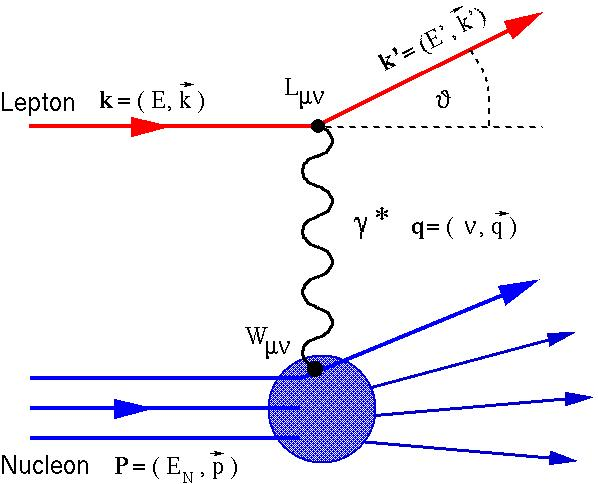
\includegraphics[width =5cm]{../images/DIS}
	\end{figure}
		
	
	\column{.5\textwidth} % Right column and width
	\begin{itemize}
		\item Momentum Transfer $ Q^2 \equiv 4EE' sin \frac{\theta}{2} $
		\item Bjorken X $(X_{bj}/x) = \frac{Q^2}{2\nu M}$
		\item $\sigma_{eN} = \frac{\alpha^2}{eE^2sin^4(\frac{\theta}{2})} [\frac{F_2}{\nu}cos^2\frac{\theta}{2} + \frac{2F_2}{M}sin^2\frac{\theta}{2}] $
		\item Invariant Mass $W^2 = 2M\nu + M^2 - Q^2$
		\item $W^2 > 4 \rightarrow$ DIS
	\end{itemize}
	

	
\end{columns}
\end{frame}
%----------------------------------------------

\section[MARATHON]{MARATHON}
\subsection{Setup}
%----------------------------------------------
\begin{frame}
\frametitle{Tritium Experiments}
	\vspace{-15pt}
	\begin{figure}
		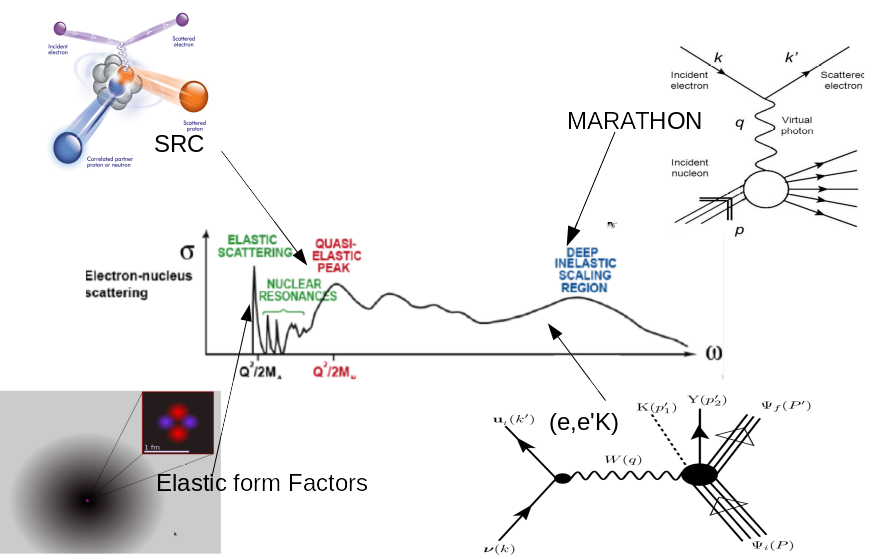
\includegraphics[width =12cm]{../images/tritium_ov}
	\end{figure}
\end{frame}

\begin{frame}
\frametitle{MARATHON}
		MeAsurement of $F^n_2/F^p_2, d/u$ RAtios and $A=3$ EMC Effect in Deep Inelastic Electron Scattering off the Tritium and Helium MirrOr Nuclei.
	\vspace{-10pt}
	\begin{columns}[t]
	
		\column{.45\textwidth} % L column and width

		\begin{figure}
			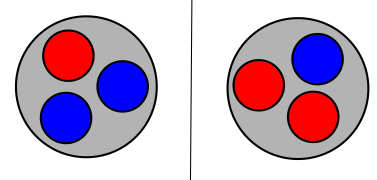
\includegraphics[width =5cm]{../images/mirror}
		\end{figure}
		\vspace{-20pt}
		\begin{figure}
			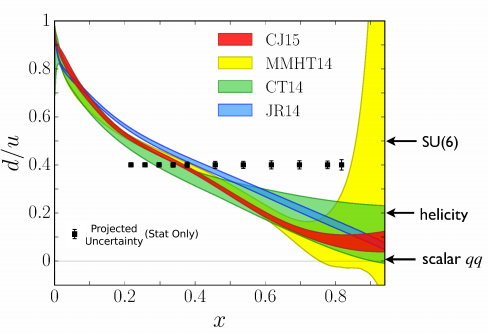
\includegraphics[width=5cm]{../images/d_u}
			\caption{d/u quark distribution ratios}
		\end{figure}

		\column{.55\textwidth} % Right column and width
		\begin{itemize}
			\item Lightest and simplest mirror system
			\begin{itemize}
				\item  Number of protons in $^3H =$ neutrons in $^3He$
	  		 \end{itemize}
			\item Differences in the nuclear effects are small
			\item Improve the current measurement and understanding of Fn2 to F p2 ratio
			\item Restrict the assumptions and parameters made in the model calculations of the down to up quark distribution ratio
		\end{itemize}


	\end{columns}
\end{frame}

%----------------------------------------------------
\begin{frame}
\frametitle{Tritium Target Cell}
\begin{columns}
	\column{0.45\textwidth}
	First tritium target at JLab
	\begin{itemize}
		\item Thin Al entrance and exit windows ~0.01 inches
		\item 1090Ci of Tritium (0.1 g)
		\item 25 cm long
		\item Tritium Cell was filled in Savannah River
		\item 40 kelvin Helium is used to cool an attached heat sink
	\end{itemize}
	\column{0.45\textwidth}
	\begin{figure}
		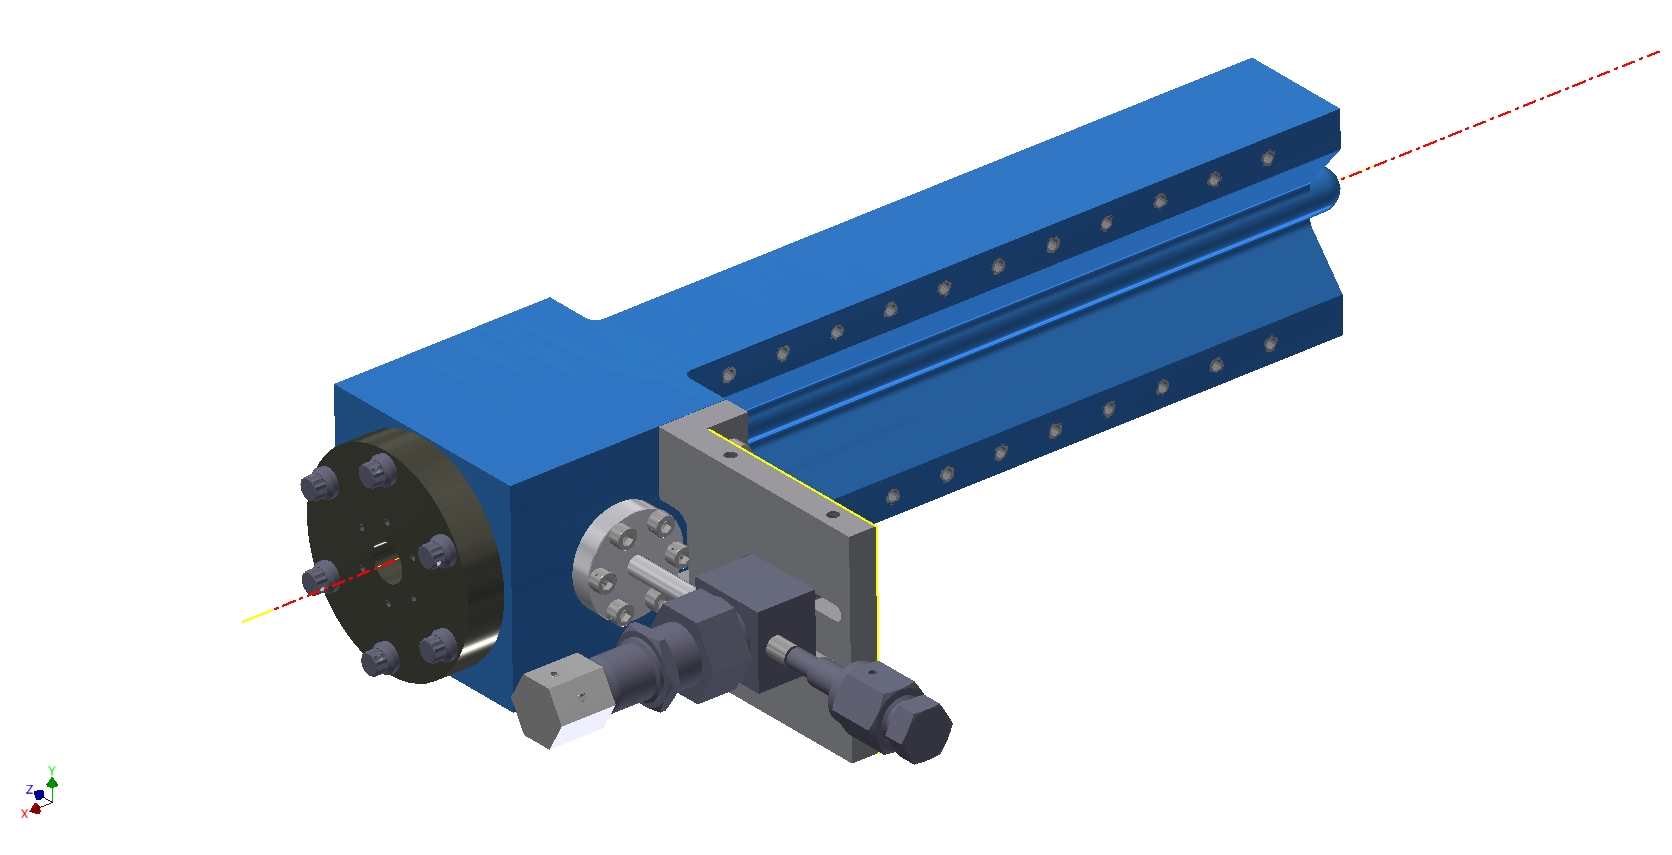
\includegraphics[width=5cm]{../images/tgt_cell}
	\end{figure}
	\vspace{-10pt}
	\begin{figure}
		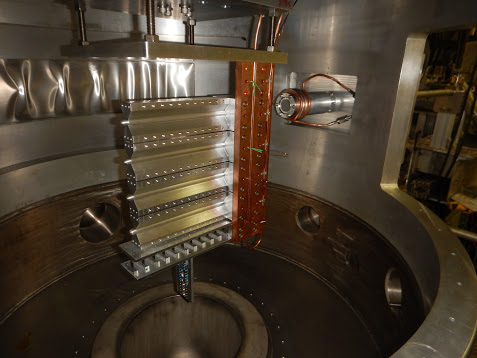
\includegraphics[width=5cm]{../images/tag_lat}
	\end{figure}
\end{columns}
\end{frame}

%------------------------------------------------

\begin{frame}
\frametitle{Hall A $\&$ The HRSs}

\begin{block}{}
	Use CEBAF(Continues Electron Beam Facility) to provide 10.6 GeV beam for electron scattering. 
\end{block}
\vspace{-20pt}
\begin{columns}
\column{0.45\textwidth}
\begin{figure}
	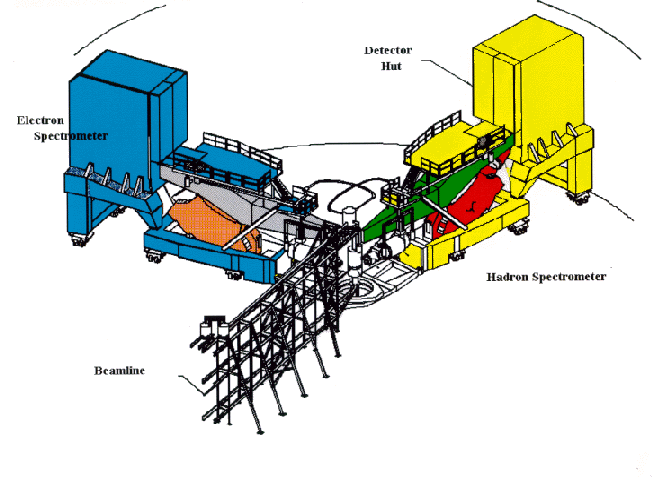
\includegraphics[width=6cm]{../images/Halla_img}
\end{figure}
\column{0.45\textwidth}
\begin{figure}
	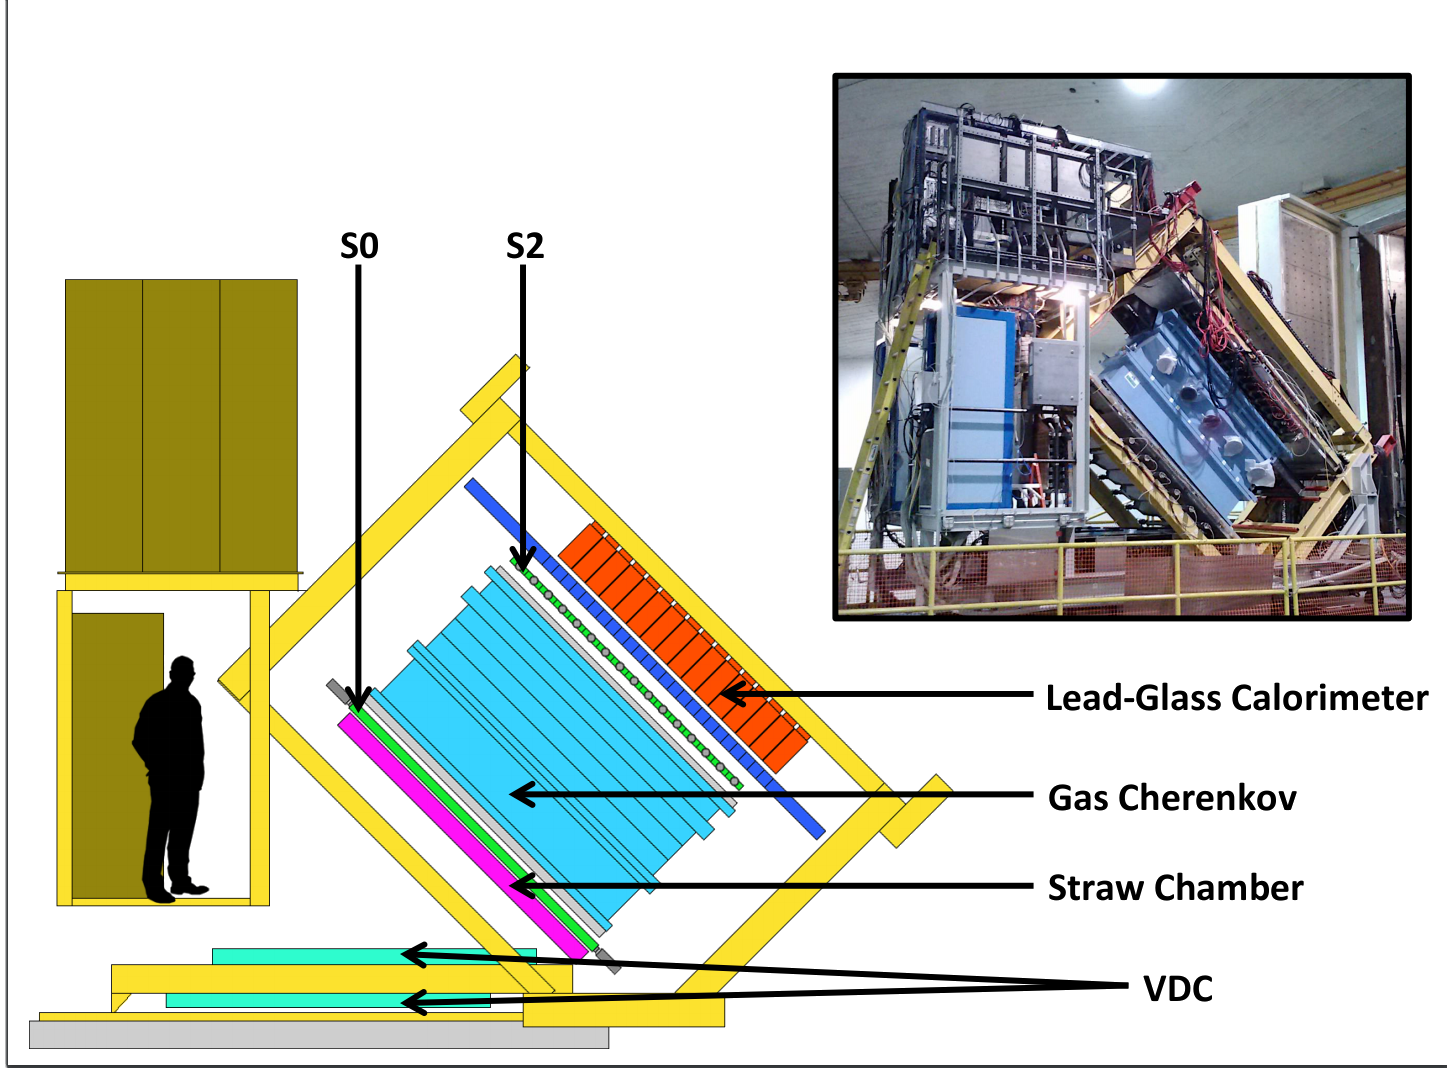
\includegraphics[width=6cm]{../images/HRS_cartoon}
\end{figure}

\end{columns}
\end{frame}
%---------------------------------------------------------------

\begin{frame}
\frametitle{Vertical Drift Chamber(VDC)}
	\begin{columns}
		\column{0.55\textwidth}
		\begin{figure}
			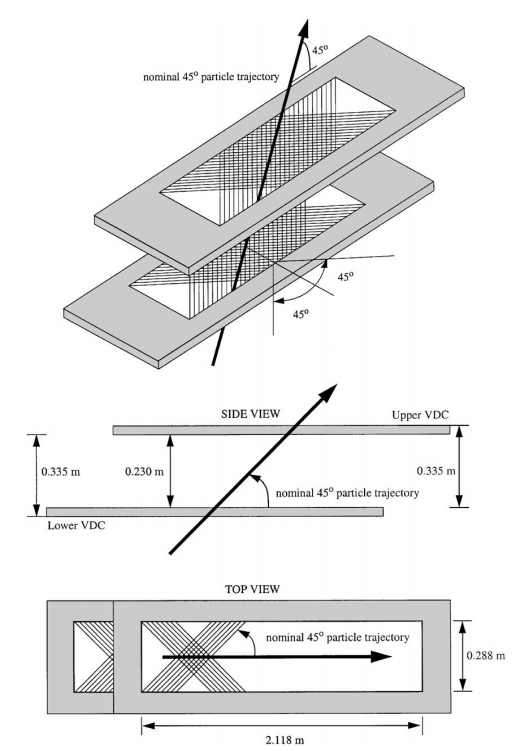
\includegraphics[width=5cm]{../images/VDC}
		\end{figure}	
				\column{0.45\textwidth}
		\begin{block}{Tracking Detector}
		A dual VDC system is used to provide precise angular reconstruction of particle trajectories.
		\begin{itemize}
			\item U/V angle $\pm 45 ^\circ$
			\item 368 wired per plane
			\item 4.2mm spacing between wires
			\item Online Efficiency determined by nearest neighbor method \cite{nim}
		\end{itemize}
	\end{block}
	\end{columns}
\end{frame}
%---------------------------------------------------------------
\begin{frame}
\frametitle{Gas Cherenkov}

	\begin{columns}
		\column{0.45\textwidth}	
		\begin{figure}
			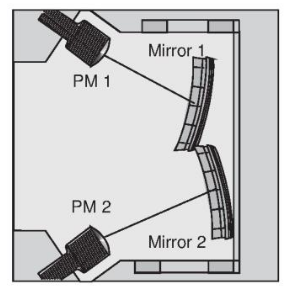
\includegraphics[width=3cm]{../images/Cher}
		\end{figure}
		\begin{figure}
			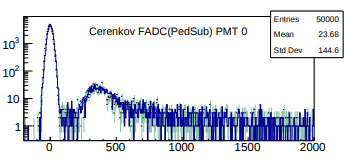
\includegraphics[width=5cm]{../images/cher_1pmt}
		\end{figure}
		\column{0.55\textwidth}
		\begin{block}{PID Detector}
		\begin{itemize}
			\item Filled with $CO_2$
			\item Index of refraction of 1.00041 and operated at 1 atm
			\item Electron threshold of 0.017 $\frac{GeV}{c}$
			\item Pion/proton threshold  of 4.8/32 $\frac{GeV}{c}$
			\item 1.5/1 m radiator length of left/right arm \cite{nim}
		\end{itemize}
		\end{block}
	\end{columns}
\end{frame}


%---------------------------------------------------------------
\begin{frame}
\frametitle{Calorimeter}

\begin{columns}[t]
	\column{0.55\textwidth}	
	\vspace{-25pt}
	\begin{figure}
		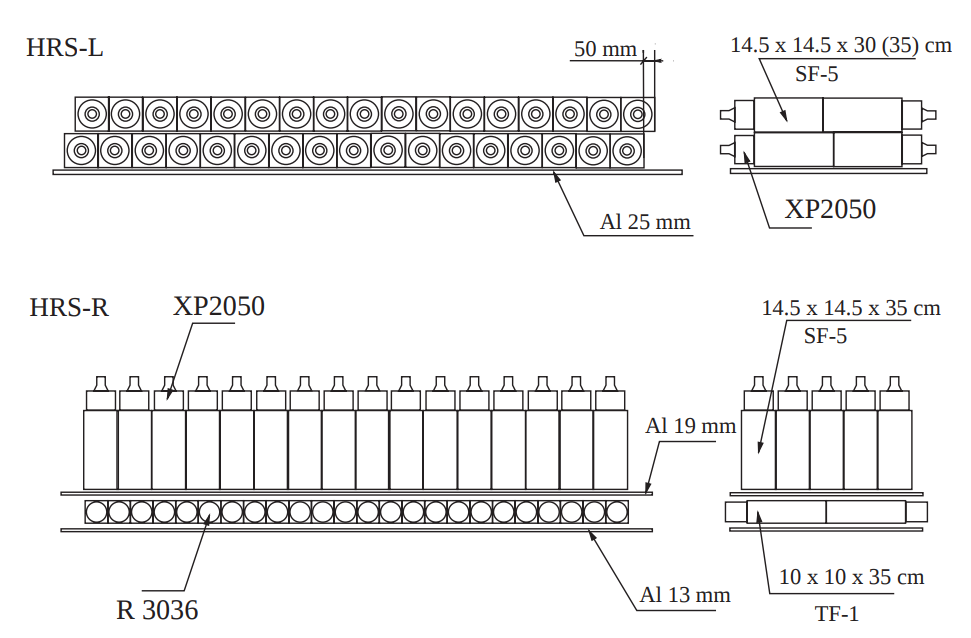
\includegraphics[width=6cm]{../images/calo}
	\end{figure}
	\vspace{-10pt}
	\begin{figure}
		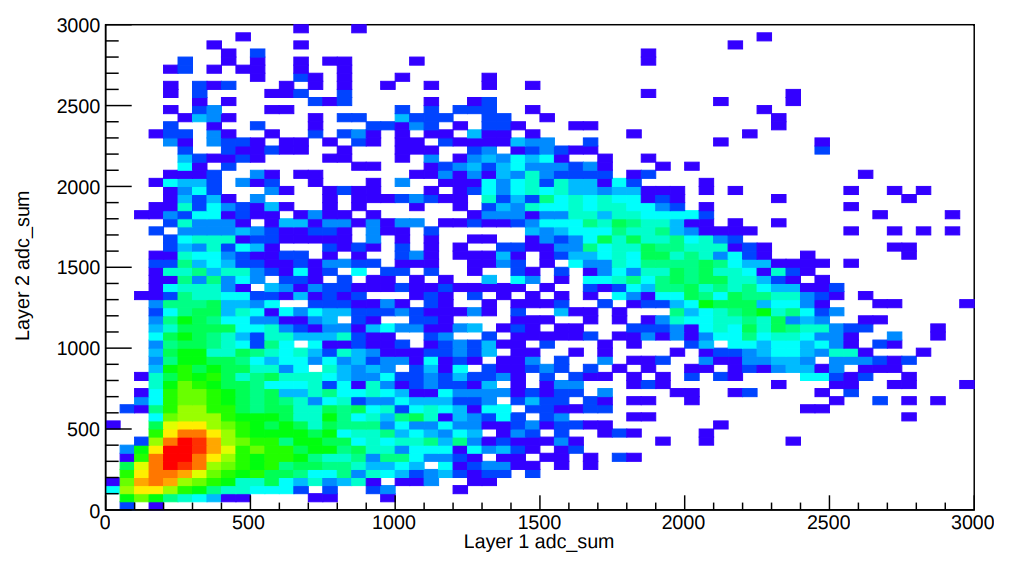
\includegraphics[width=6cm]{../images/PR1_2}
	\end{figure}	

	\column{0.5\textwidth}
	\begin{block}{PID Detector}
	\begin{itemize}
		\item Two layers of lead glass
		\item LHRS -Both layers are stacked perpendicular to beam direction.
		\vspace{-13pt}
 		\begin{itemize}
			\item 48 Blocks, 80 blocks
		\end{itemize}
		\item RHRS -First layer perpendicular, second layer is parallel
		\begin{itemize}
			\item 34 Blocks, 34 blocks
		\end{itemize}
		\item With Chernenkov, pion suppression above 2$\frac{GeV}{c}$ of a factor of $2e5$ \cite{nim}
	\end{itemize}
	\end{block}
\end{columns}
\end{frame}


%---------------------------------------------------------------

\begin{frame}
\frametitle{Scintillators}
\vspace{-8pt}
	\begin{columns}
		\column{0.45\textwidth}
		\begin{block}{Triggering Detector}
			\begin{itemize}
				\item Two Scintillating light detectors
				\begin{itemize}
					\item S0 large acceptance and low resolution
					\item S2 16 bars capped by PMTs
				\end{itemize}
				\item Main source for trigger
				\item Provide TOF(time of flight) $\&$ Used to help identify hadrons \cite{nim}
			\end{itemize}
		
		\end{block}
	\column{0.45\textwidth}
		\begin{figure}
			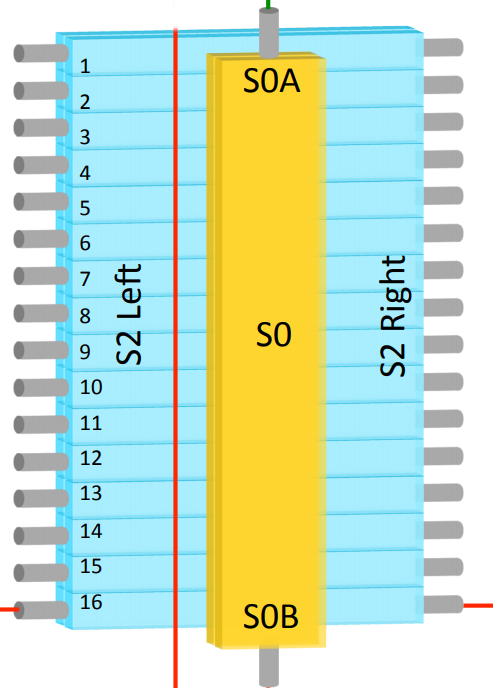
\includegraphics[width=5cm]{../images/Scins}
		\end{figure}
	\end{columns}
\end{frame}

%---------------------------------------------------------------
\begin{frame}
\vspace{-8pt}
\begin{figure}
	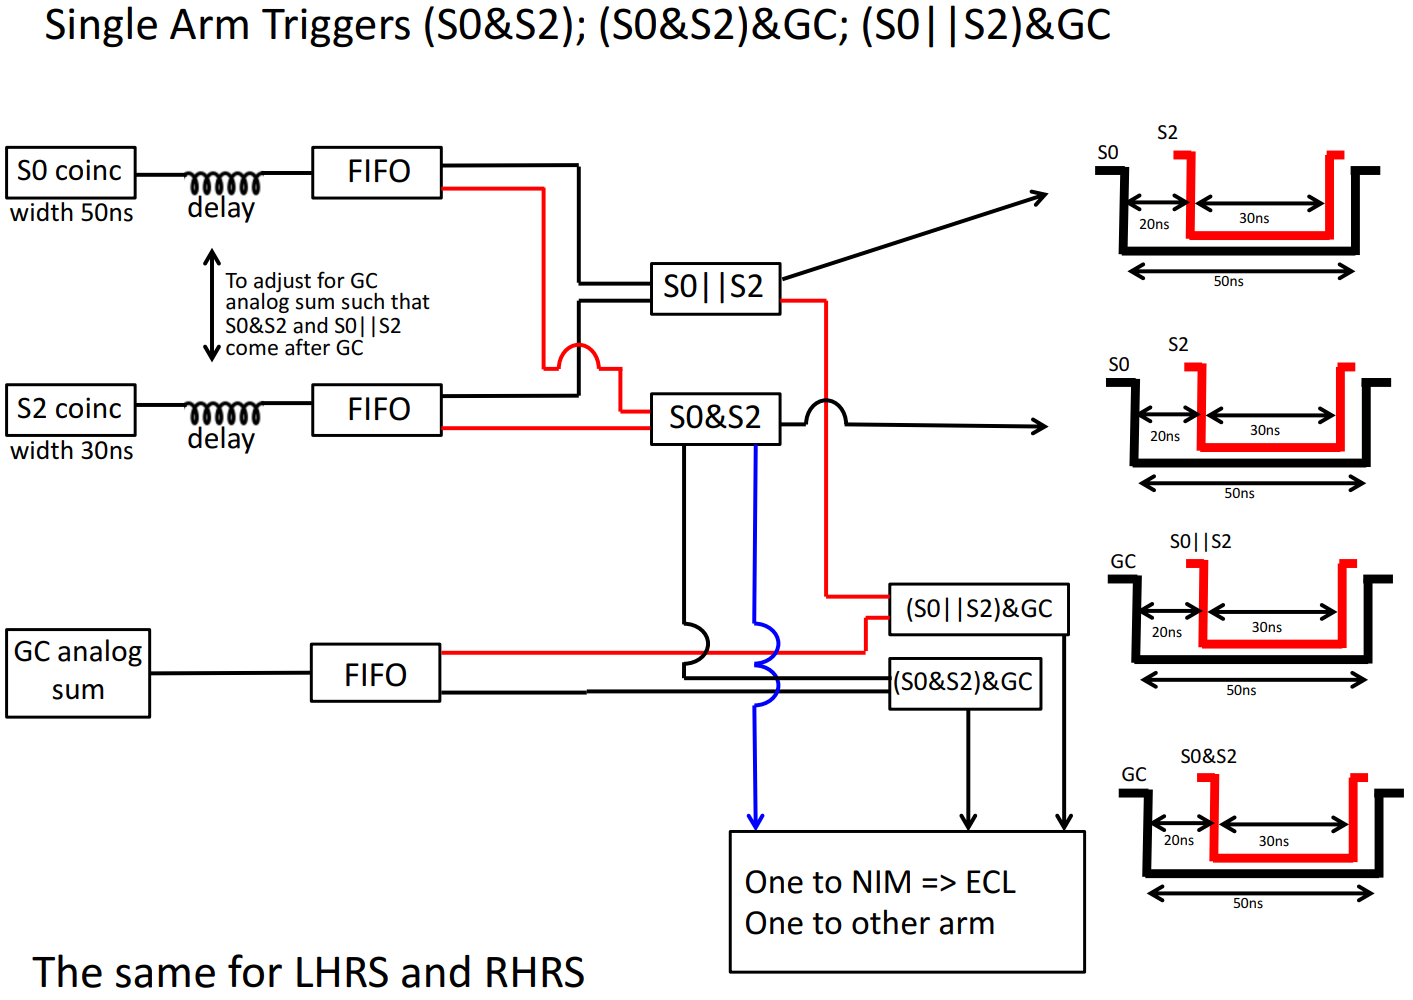
\includegraphics[width=12cm]{../images/trigger_1}
	\caption{By Florian Hauenstein}
\end{figure}
\end{frame}


%---------------------------------------------------------------


\subsection{Run Period}

\begin{frame}
\frametitle{The Run Period}
	\vspace{-20pt}
	\begin{columns}
		\column{0.35\textwidth}	
		\begin{figure}
			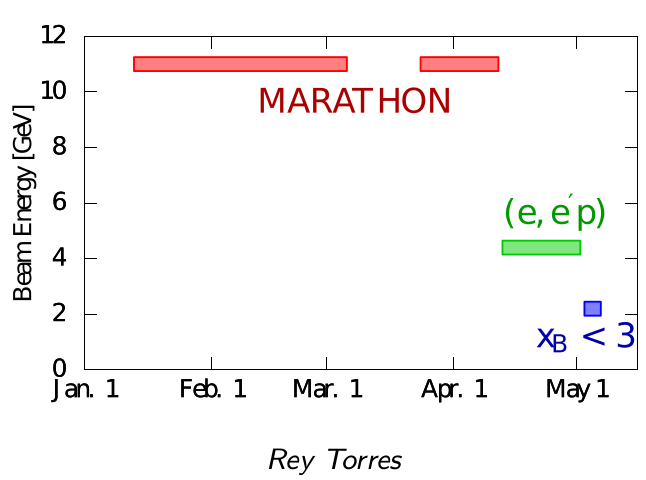
\includegraphics[width=4.5cm]{../images/run_per}
		\end{figure}
		\column{0.65\textwidth}
		\vspace{-10pt}
		\begin{itemize}
			\item Ran from January 11th to April 12th of 2018.
			\item Gaseous Tritium, Deuterium, Helium-3, and Hydrogen
			\item Single Carbon Foil, Carbon foil with hole, and multi-foil
			\item Rotated through targets to achieve equal statics and reduce the impact of unforeseen circumstances
		\end{itemize}
	\end{columns}
	\begin{figure}
	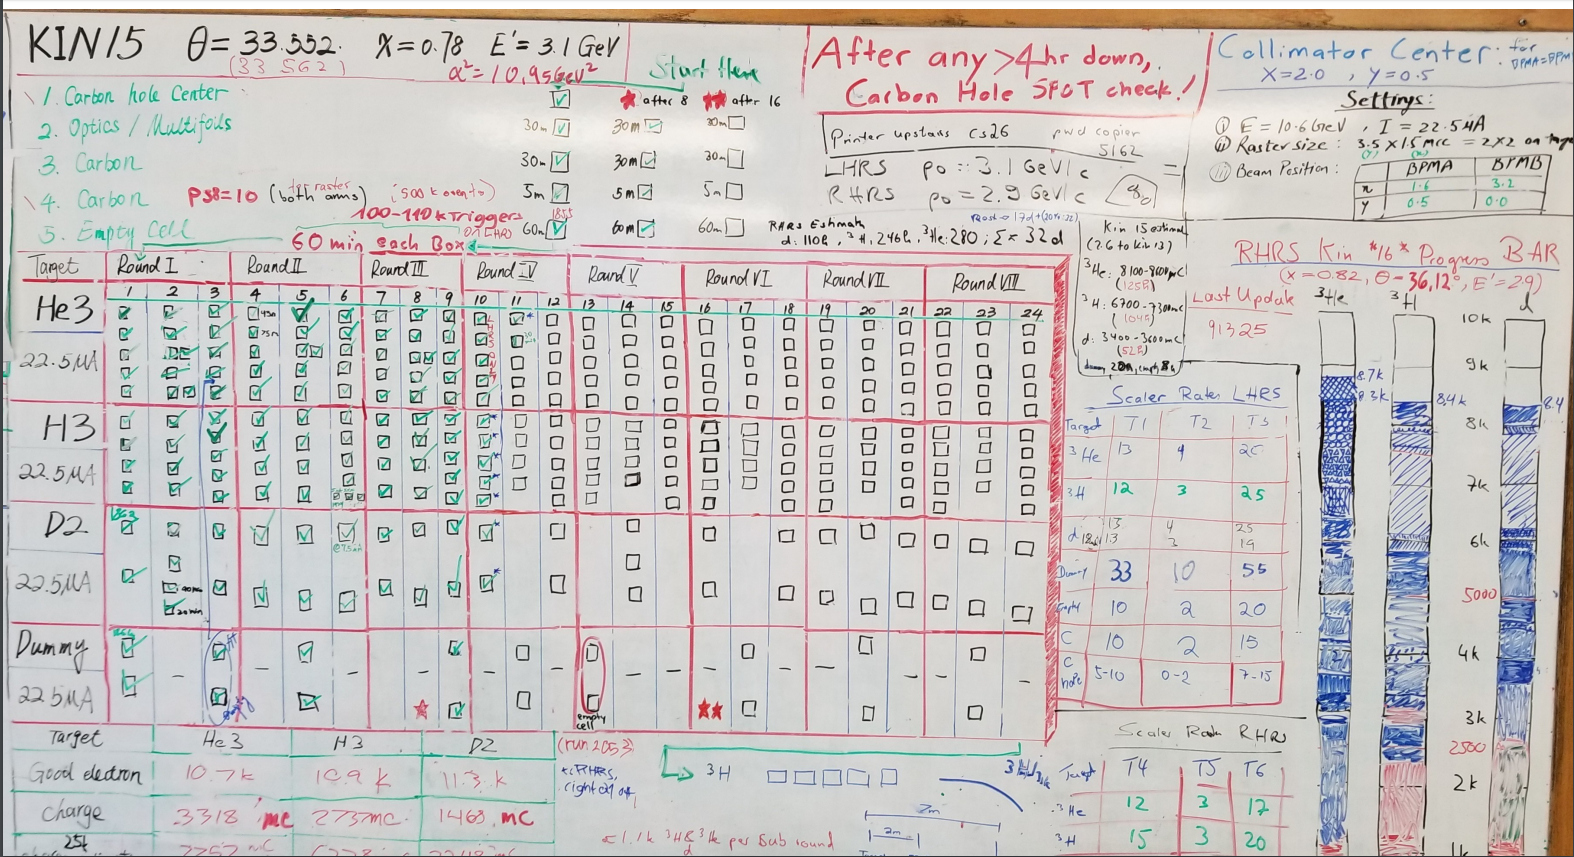
\includegraphics[width=6.5cm]{../images/whiteboard_2_20}
	\end{figure}
\end{frame}

%--------------------------------------------------------
\begin{frame}
\frametitle{Major Miscues}
\begin{block}{}
	\begin{itemize}
		\item Right Arm Dipole failed on January 11th
		\begin{itemize}
			\item Return the dipole to functionally the following day
			\item 01/13 - Dipole failed again, causing a chain reaction with the Left arm
			\item Solution could not be found quickly
			\item Change of Kinematic plan to use single HRS.
			\item Recovered RHRS on 01/16 - Set to take data at theta of 36.12$^\circ$,  $x$ of 0.82 
		\end{itemize}
		\item A Transformer Failed on March 5th 
		\begin{itemize}
			\item Recovered on March 23rd
			\item Spring run Period extended by 18 days
			\item MARATHON took opportunistic data during recovery period 
		\end{itemize}
	\end{itemize}
\end{block}

\end{frame}
%------------------------------------------------------------------

\begin{frame}
\begin{columns}[t]
	\column{0.55\linewidth}
%	\vspace{-10pt}
	
	\begin{figure}
		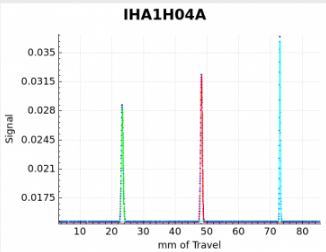
\includegraphics[width=4.5cm]{../images/harpscan1}
	\end{figure}
	
	\vspace{-10pt}
	\begin{figure}
		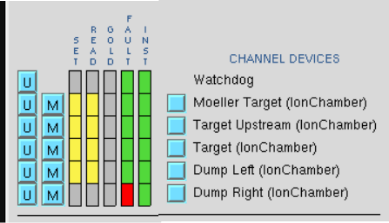
\includegraphics[width=4.5cm]{../images/ION}
	\end{figure}
	\column{0.5\linewidth}
	\vspace{-20pt}
	\begin{block}{Tritium Safety Requirements}
		\begin{itemize}
			\item Harp and BPM Check!
			\item Ion Chamber functionality test
			\item Beam Center
			\item Raster Size calibration. 
		\end{itemize}	
	\end{block}	
	\vspace{-10pt}
	\begin{figure}
		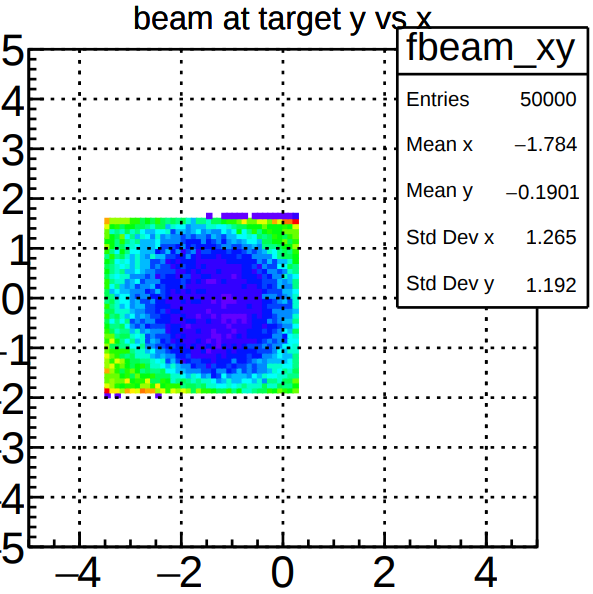
\includegraphics[width=5cm]{../images/spot}
	\end{figure}	
\end{columns}
\end{frame}
%------------------------------------------------------------------
\begin{frame}
	\begin{columns}[c]
	\column{0.45\textwidth}
	\begin{block}{Shift Crew Task}
		\begin{itemize}
			\item Monitor Detector plots 
			\item Record and observe event frequency
			\item Observe target response including the temperature sensor attached to the target ladder.
		\end{itemize}
	\end{block}

	\column{0.55\textwidth}

	\vspace{-40pt}
	\begin{figure}
		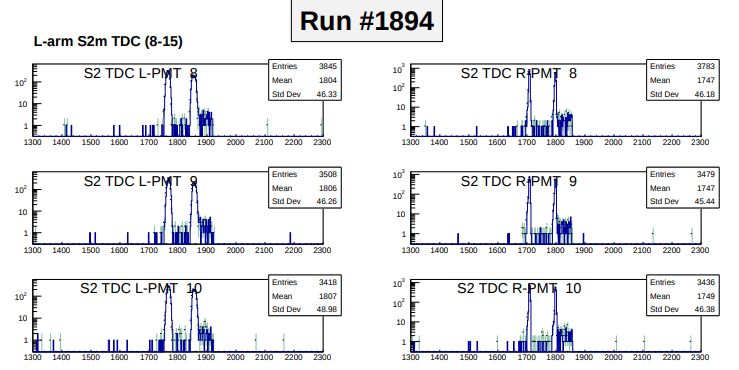
\includegraphics[width=6cm]{../images/OnlineGui}
	\end{figure}
	\vspace{-20pt}
	\begin{figure}
		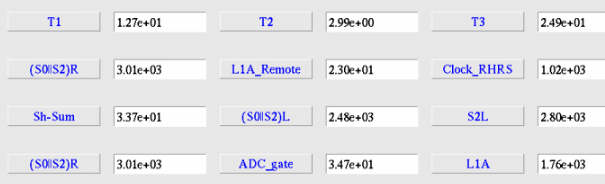
\includegraphics[width=5cm]{../images/scaler}
	\end{figure}
	\vspace{-20pt}
	\begin{figure}
		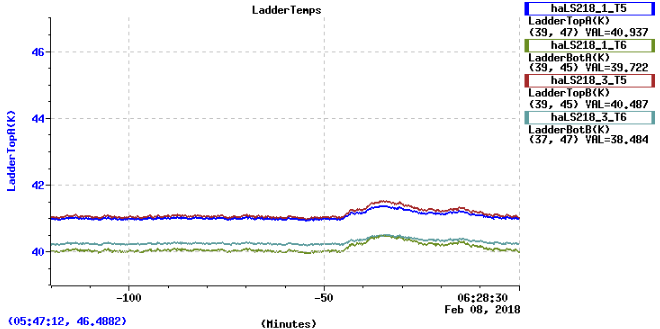
\includegraphics[width=5cm]{../images/lattertmps_g}
	\end{figure}
	
\end{columns}
\end{frame}

%----------------------------------------------------------------------------

\section[Analysis]{Analysis}

\begin{frame}
\frametitle{Analysis}
	\begin{columns}
	\column{0.45\textwidth}
	\begin{block}{Data Analysis Task}
		\begin{itemize}
			\item Data decoding 
			\item Online analysis
			\item Full detector calibrations 
			\item Detector efficiencies
			\item Systematic Studies
		\end{itemize}
	\end{block}
	\column{0.45\textwidth}
	\begin{block}{Monte Carlo Analysis}
		\begin{itemize}
			\item Monte Carlo Tunning
				\begin{itemize}
					\item Offsets
					\item Target Parameters
					\item Reconstruction functions
				\end{itemize}
			\item Event weighting 
			\item Acceptance studies
			
		\end{itemize}
	\end{block}
	\end{columns}
	\begin{block}{}
		\begin{itemize}
			\item Cross section extraction through Data to Monte Carlo ratio method
			\item Application of Nuclear Corrections
			\item Compare Cross Section of A=3 Nuclei to that of Deuterium to calculate EMC effect 
		\end{itemize}
	\end{block}
\end{frame}
%------------------------------------------------------------------ 
\begin{frame}
\frametitle{Data Decoding}
\vspace{-5pt}
\begin{block}{The Hall A Analyzer}
	\begin{itemize}	
		\item An object-oriented, modular framework built on top of ROOT. 
		\item Use modular classes to build a detector package 
		\item Libraries to calculate physics variables 
	\end{itemize}
	\begin{columns}
		\column{0.55\textwidth}
		\begin{itemize}
			\item THaRasterBeamClass
			\item THaCherenkov
			\item THaTrackingDetector
		\end{itemize}
		\column{0.55\textwidth}
		\begin{itemize}
			\item Tri$\_$Beam$\_$Eloss
			\item TriBCM
			\item TriFADCBPM
		\end{itemize}		
	\end{columns}
\end{block}
\vspace{-190pt}
\begin{figure}
	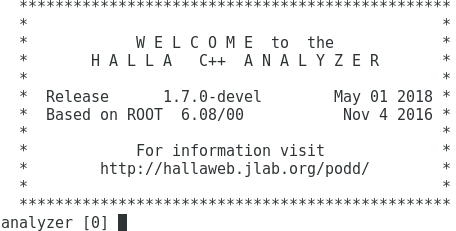
\includegraphics[width=4cm]{../images/ana}
\end{figure}
\vspace{90pt}
\begin{columns}
	\column{0.5\textwidth}
	\begin{figure}
		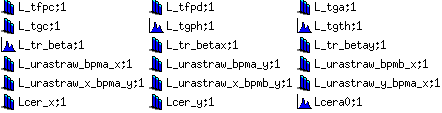
\includegraphics[width=6cm]{../images/histos}
	\end{figure}
	\column{0.5\textwidth}
	\begin{figure}
		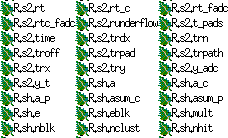
\includegraphics[width=4cm]{../images/branches}
	\end{figure}
\end{columns}

\end{frame}

%------------------------------------------------------------------

\begin{frame}
\frametitle{Online Analysis}
\begin{block}{}
\begin{columns}
\column{0.45\textwidth}

		\begin{itemize}
			\item Quick Calibrations
			\item Electron Counts
			\item Comparable plots for detector checks
		\end{itemize}

	\begin{figure}
		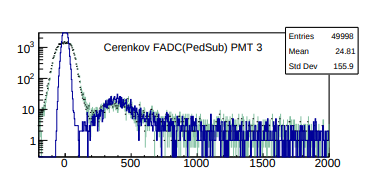
\includegraphics[width=5cm]{../images/det_check}
	\end{figure}

\column{0.45\textwidth}	
	\begin{figure}
		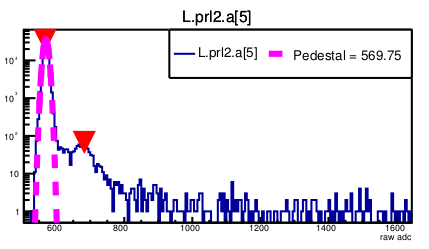
\includegraphics[width=5cm]{../images/cer_ped}
	\end{figure}
	\vspace{-20pt}
	\begin{figure}
		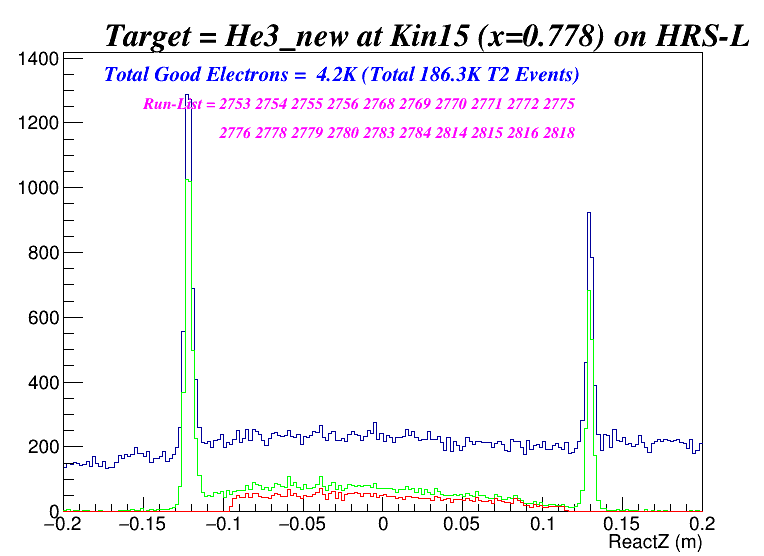
\includegraphics[width=5cm]{../images/G_E}
	\end{figure}

\end{columns}
\end{block}
\end{frame}
%------------------------------------------------------------------


\begin{frame}

	\vspace{-1pt}
	\begin{block}{Detector Calibrations}
		\vspace{-10pt}
		\begin{columns}[]
			\column{0.5\textwidth}
				\begin{figure}

					\caption{BCM calibration}
					\vspace{-20pt}
					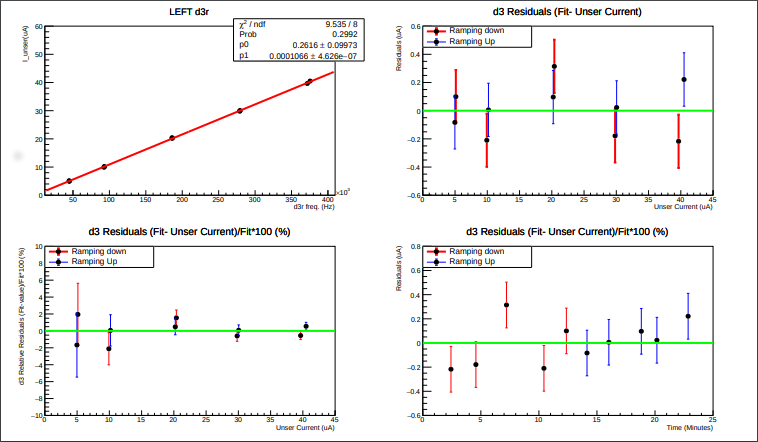
\includegraphics[width=7cm]{../images/BCM_cal_nb}
				\end{figure}
				\column{0.5\textwidth}
				\vspace{-20pt}

				\begin{figure}
					
					\caption{Gain and Pedestal calibration}
						\vspace{-10pt}
					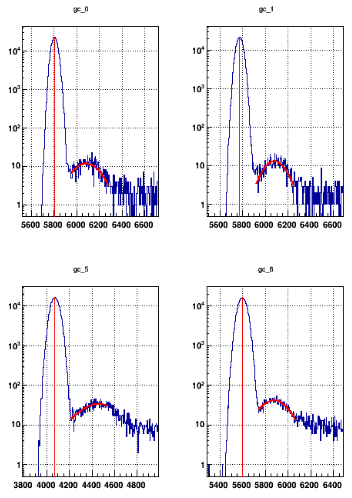
\includegraphics[width=5cm]{../images/GC_cal}
				\end{figure}

		\end{columns}
	\end{block}
	
	
\end{frame}

%------------------------------------------------------------------
\begin{frame}

\begin{block}{Detector Calibrations}
\begin{figure}
	\caption{Beta calibration}
	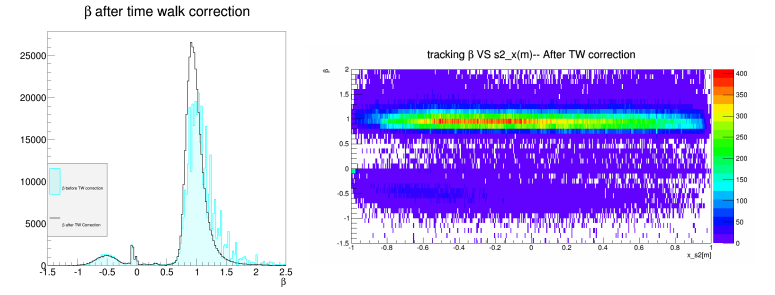
\includegraphics[width=8.5cm]{../images/beta_cal}
\end{figure}
\vspace{-15pt}
\begin{figure}
	\caption{Calorimeter Energy Calibration}
	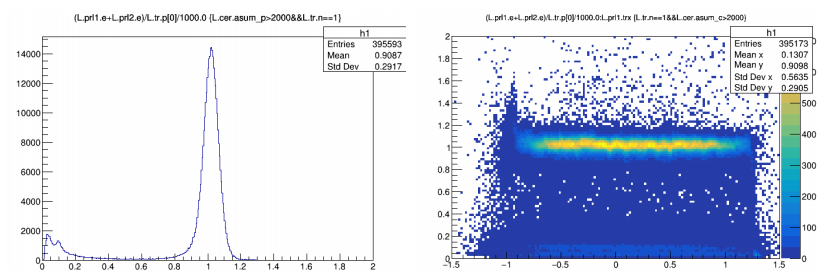
\includegraphics[width=8.5cm]{../images/e_cal}
\end{figure}

\end{block}	
\end{frame}

%------------------------------------------------------------------
\begin{frame}{BPM Calibration}
	\vspace{-30pt}
	\begin{columns}
		\column{0.45\textwidth}
		\begin{figure}
			\caption{Harp Scan}
			\vspace{-20pt}
			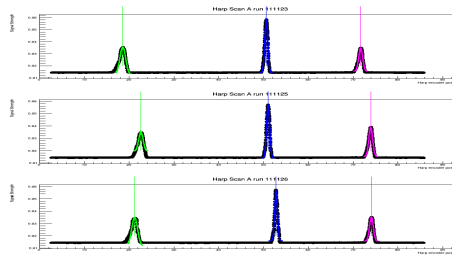
\includegraphics[width=5.5cm]{../images/harpscan}
		\end{figure}
			\column{0.45\textwidth}
		\vspace{-10pt}
		\begin{figure}
			\caption{BPM pedestals}
			\vspace{-2pt}
			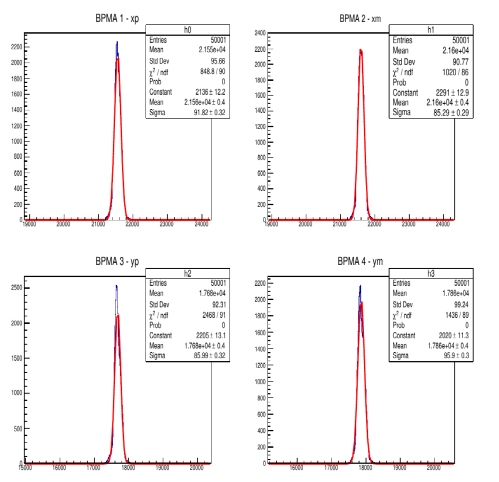
\includegraphics[width=4.5cm]{../images/BPM_ped}
		\end{figure}
	\end{columns}
	\vspace{-10pt}
	\begin{figure}
		\caption{ Before and After}
		\vspace{-5pt}
		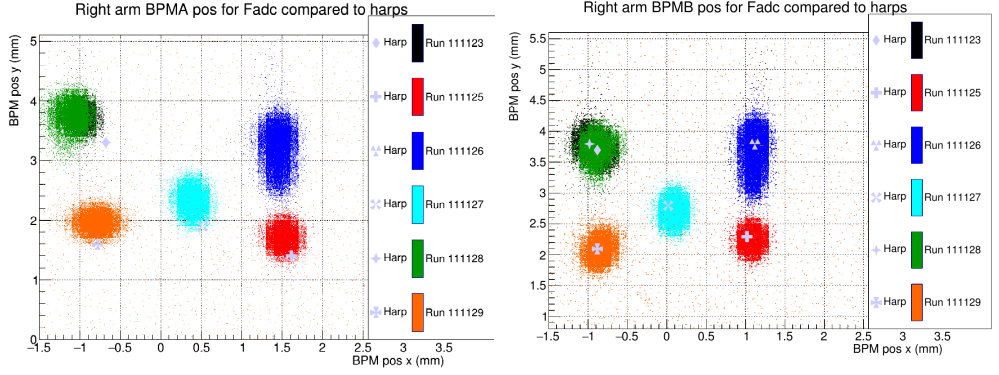
\includegraphics[width=8cm]{../images/BPM_b_a}
	\end{figure}

\end{frame}
%------------------------------------------------------------------
\begin{frame}{Efficiencies}
	\begin{columns}

		\column{0.35\textwidth}
		\vspace{-80pt}
		\begin{itemize}
			\item Particle ID
			\item Tracking Efficiency
			\item Dead Time
			\item Trigger Efficiency
			
		\end{itemize}			
			
	\column{0.75\textwidth}
	\vspace{-40pt}
	\begin{figure}
		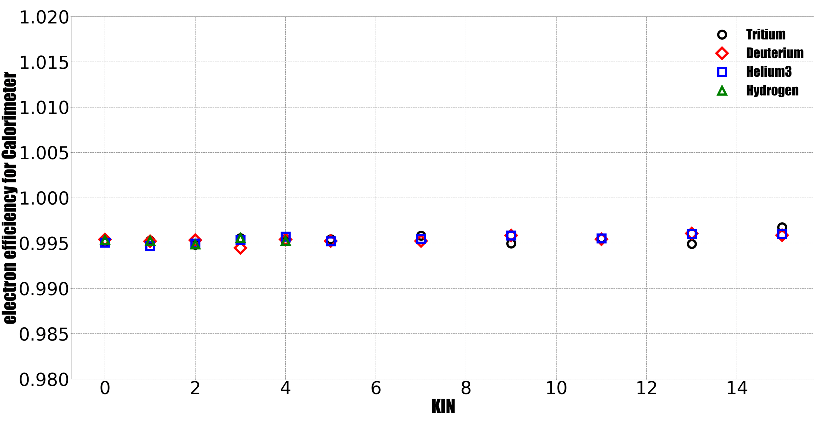
\includegraphics[width=7cm]{../images/pid_eff}
	\end{figure}
	\vspace{-25pt}
	\begin{figure}
		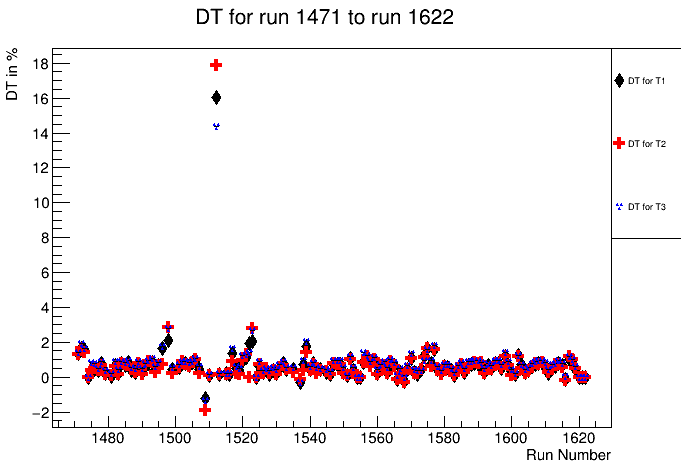
\includegraphics[width=7cm]{../images/DT}
	\end{figure}
	\end{columns}
\end{frame}
%------------------------------------------------------------------
\begin{frame}{Systematic Studies}
	\vspace{-20pt}
	\begin{columns}
		\column{0.45\textwidth}	
		\begin{figure}\caption{Density Fluctuations}\vspace{-10pt} 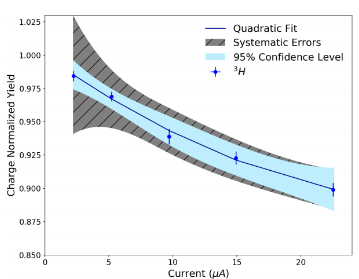
\includegraphics[width=5cm]{../images/dens}\end{figure}
		\vspace{-10pt}
		\begin{figure}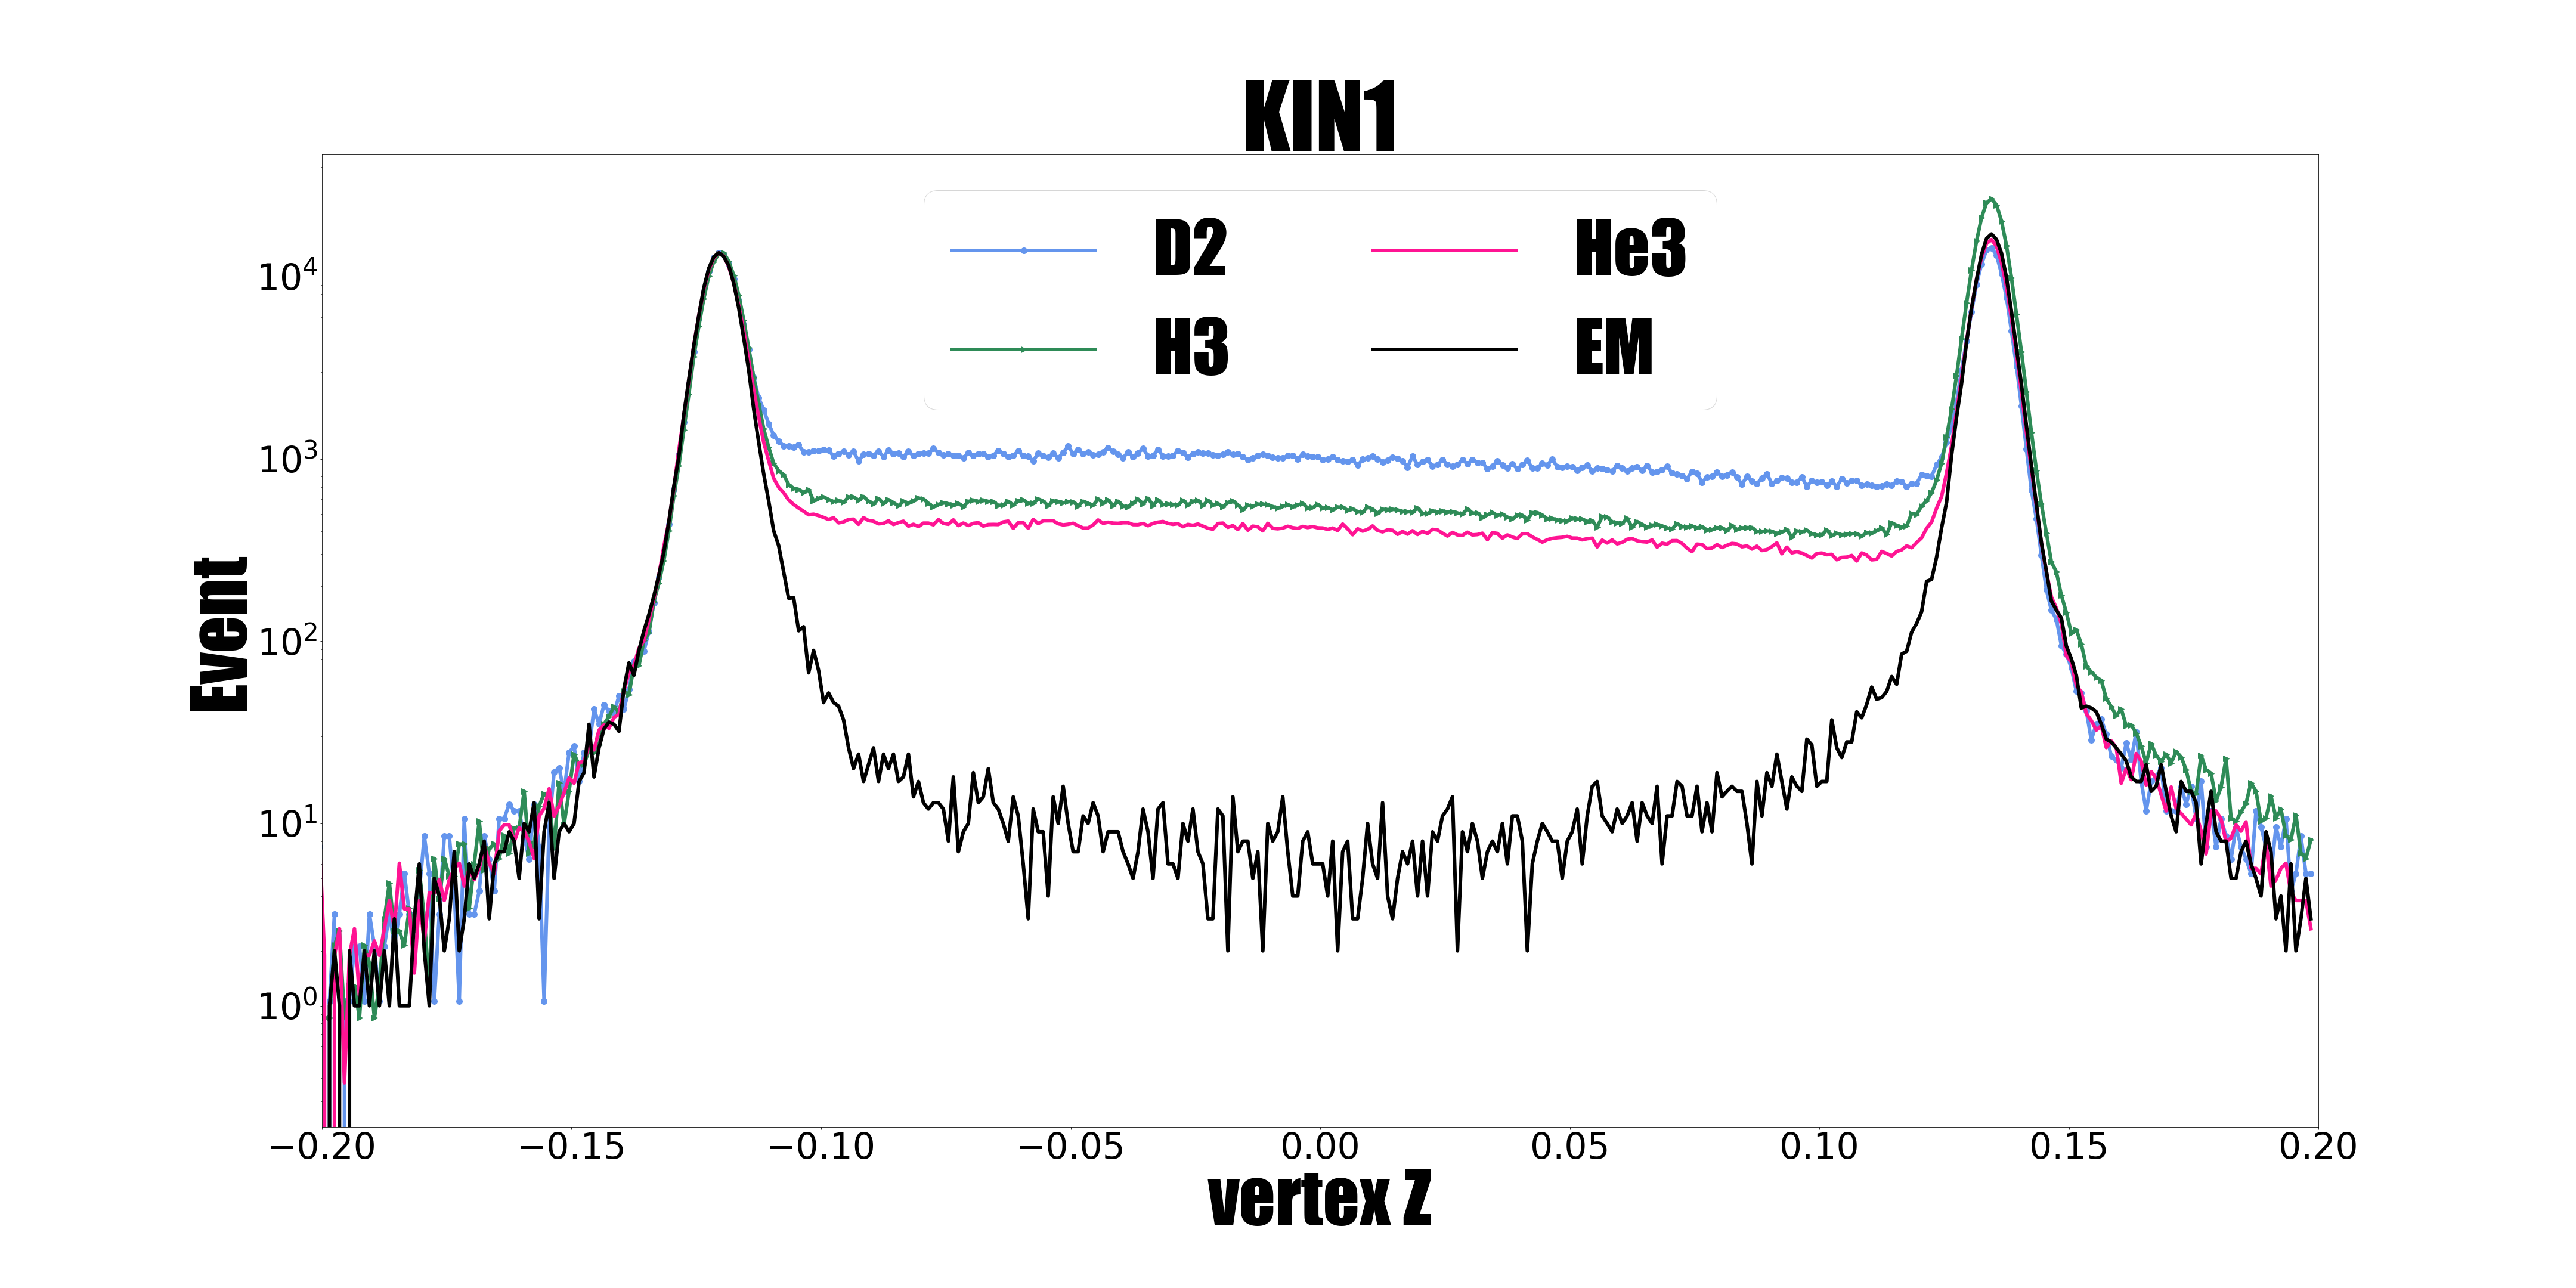
\includegraphics[width=5cm]{../images/ecc}
		\caption{End Cap Contamination}\end{figure}
		\column{0.55\textwidth}	
		\begin{figure}\caption{Tritium beta decay} 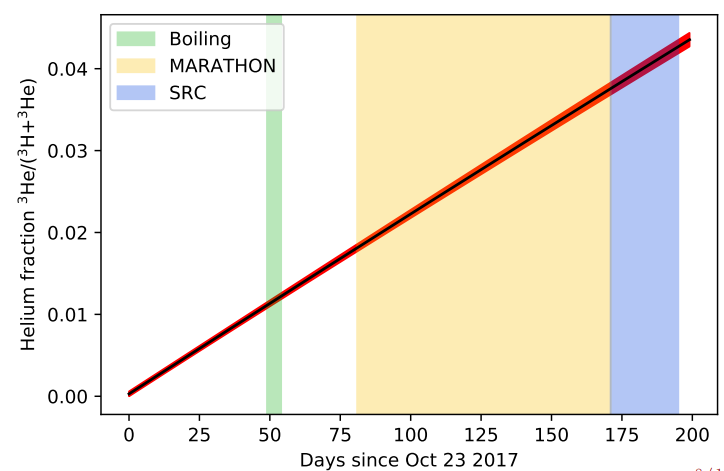
\includegraphics[width=5cm]{../images/decay}\end{figure}
		\vspace{-10pt}
		\begin{figure}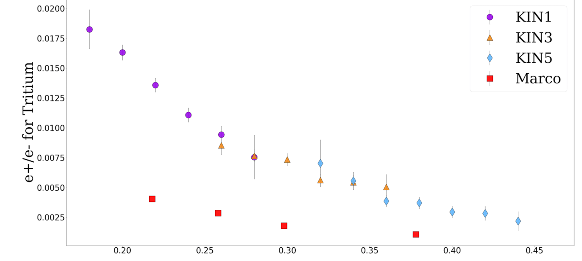
\includegraphics[width=5cm]{../images/pos}
		\caption{Charge Symmetric background}\end{figure}
	\end{columns}
\end{frame}
%------------------------------------------------------------------
\begin{frame}{}
\begin{columns}
\column{0.5\textwidth}
		\begin{block}{Monte Carlo}
			\begin{itemize}
				\item Generate events in target space
				\item Pass through detector aperture
				\item Use optics matrix to project back to target from focal plane.
				\item Tune Simulation to match detector response
				\item Adjust initial parameters
				\item Use model to weight events
				\begin{itemize}
					\item Deep Inelastic Bodek Fit \cite{bodek}
					\item Quasi elastic  and elastic  
				\end{itemize}    
			\end{itemize}
		\end{block}
\column{0.45\textwidth}
	\vspace{-20pt}
	\begin{figure}
		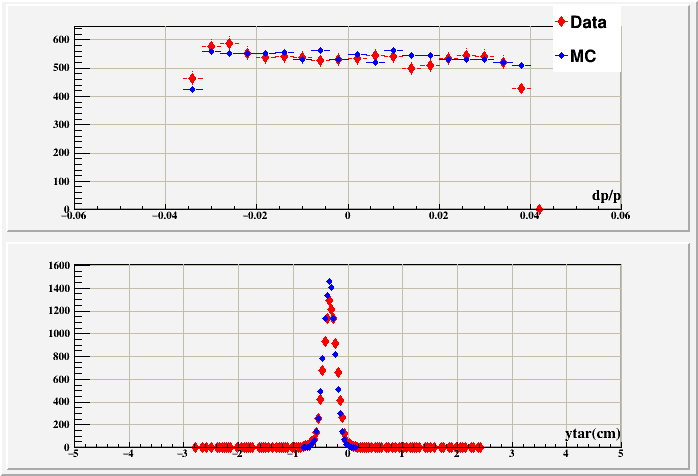
\includegraphics[width=6cm]{../images/dp_ytar_1207.png}
	\end{figure}
	\vspace{-30pt}
	\begin{figure}
		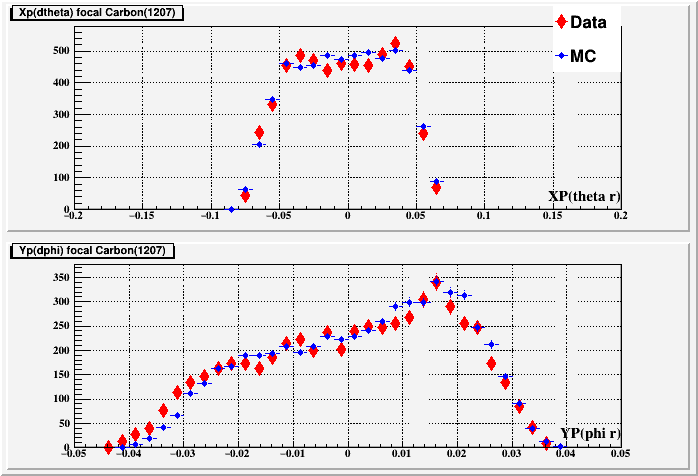
\includegraphics[width=6cm]{../images/xp_yp_foc_1207.png}
	\end{figure}
\end{columns}
\end{frame}




%------------------------------------------------------------------
\begin{frame}{Cross Section}
	\begin{block}{}
		\centering
		 $N_e = \textit{L} * \left( \frac{d\sigma}{d\Omega dE^\prime} \right) * \left( \Delta E^\prime \Delta \Omega\right) \epsilon * A \left(E^\prime \theta \right)  + Back  Ground$
		
		\begin{itemize}
			\item $\textit{L}$ Luminosity $\equiv$ \# of electrons per scattering centers
			\item $\left( \Delta E^\prime \Delta \Omega\right) = $ Phase space
			\item $\epsilon = $ efficiencies
			\item  $A \left(E^\prime \theta \right) =$ Acceptance 
			
		\end{itemize}
		
		$ Yield_{data} = \frac{\left(N_e - BackGround\right)}{Efficency } =  \textit{L} *\sigma^{data} * \left( \Delta E^\prime \Delta \Omega\right)*  A \left(E^\prime \theta \right)$
		
		$ Yield_{MC} = \textit{L} *\sigma^{mod} * \left( \Delta E^\prime \Delta \Omega\right)*  A \left(E^\prime \theta \right)$
	\end{block}



	\begin{center}

	\begin{block}{}
		Cross section by Monte carlo ratio  method:
\centering $ \frac{d\sigma}{d\Omega dE^\prime} = \sigma^{mod} * \left[\frac{Yield_{data} \left( 
E^\prime,\theta\right)} {Yield_{MC}\left(E^\prime,\theta\right)}\right] $

	\end{block}	
	\end{center}



\end{frame}
%------------------------------------------------------------------
\begin{frame}

\end{frame}

%------------------------------------------------------------------
\begin{frame}
	\begin{block}{Timeline}
		\vspace{-5pt}
		\parallelitem{Calibrations}{Done}
		\vspace{-5pt}
		\parallelitem{Monte Carlo Tunning $ \approx 85 \%$}{ January 2019}
		\vspace{-5pt}
		\parallelitem{Detector Efficiencies $ \approx 50 \%$}{ February 2019}
%		\hspace{10pt}	
		\vspace{-8pt}	
		\begin{columns}
		\column{0.25\textwidth}
		\begin{itemize}
			\item PID is done
		\end{itemize}
		\column{0.65\textwidth}
		\begin{itemize}
			\item Tracking, Trigger .... WIP
		\end{itemize}
		\end{columns}
		\vspace{-10pt}
		\parallelitem{Systematic Studies $ \approx 50 \%$  Need to focus on error estimation.}{ February 2019}
		\vspace{-5pt}
		\parallelitem{Acceptance Studies using Monte Carlo $ \approx 75 \%$ Finish tunning to move forward}{Feb. - March 2019}
		\vspace{-5pt}
		\parallelitem{Extraction of Cross section $ \approx 50 \%$ }{May-June 2019}
		\vspace{-5pt}
		\parallelitem{Application of Nuclear Corrections $ \approx 5 \%$}{July 2019}
		\vspace{-5pt}
		\parallelitem{Calculation of the EMC effect in A=3 nuclei $ \approx 25 \%$ }{July - August 2019}
		\vspace{-5pt}	
		\parallelitem{Thesis First Draft $ \approx 25 \%$}{August -Sept. 2019}
		\vspace{-5pt}
		\parallelitem{\textbf{Defend by November 1st$^*$!!!!!}}{\textbf{\underline{Graduate}}}
			

	\end{block}		
	
\end{frame}



%------------------------------------------------------------------

\begin{frame}
\frametitle{References}
\footnotesize{
\begin{thebibliography}{99} % Beamer does not support BibTeX so references must be inserted manually as below
\bibitem[Higinbotham D., 2013]{cc} Douglas Higinbotham (2013) 
\newblock The EMC effect still puzzles after 30 years
\newblock \emph{Cern Courier} April 2013.

\bibitem[J. Gomez et al., 1994]{slac_emc} J. Gomez et al. (SLAC-E139)  
\newblock \emph{Phys. Rev D}  49 (1994) 4348 

\bibitem[J.Seely, A. Daniel et al]{E3103} J.Seely, A. Daniel et al (2013) 
\newblock New Measurements of the EMC Effect in Very Light Nuclei
\newblock \emph{nucl-ex/0904.4448}.

\bibitem[J. Alcorn et al.]{nim} J. Alcorn et al, (2004)
\newblock Basic instrumentation for Hall A at Jefferson Lab
\newblock NIM A 522(2004) 294-346
\bibitem[A. Bodek and U.K. Yang]{bodek} A. Bodek and U.K. Yang
\newblock Nuclear Physics B, Procc. Suppl. Fall (2002) 

\end{thebibliography}
}
\end{frame}
%------------------------------------------------

\begin{frame}
\Huge{\centerline{The End}}
\end{frame}

%------------------------------------------------------------------------------------


%------------------------------------------------------------------
\begin{frame}{backup}

\end{frame}
%------------------------------------------------------------------
\begin{frame}

\end{frame}



\end{document} 
